\section{Jatkotutkimusaiheita}\label{jatko}

Luvussa \ref{tulokset} selvisi, että pistedatan kompressoiminen johtaa pienempien tiedostokokojen lisäksi myös oktettipuun rakentamisen nopeutumiseen. Toisaalta kompression purkaminen vie laskenta-aikaa visualisointivaiheessa. Laitossuunnitteluohjelmistossa tallennustilan tehokas käyttö ja pistepilven saaminen nopeasti katsottavaksi ovat tärkeää, joten olisi syytä tutkia, saadaanko kompression purkamista nopeutettua. Yksi mahdollisuus olisi säikeistää pisteiden lataamista niin, että yksi säie lukee pisteitä levyltä, toinen purkaa niiden kompressiota ja kolmas kopioi niitä näytönohjaimen muistiin.

Oktettipuun solmujen järjestäminen ruudulle projisoidun koon mukaan vie runsaasti laskenta-aikaa, minkä johdosta luvussa \ref{render} esitetty visualisointialgoritmi suoriutui heikosti suoraviivaiseen puskurivirralla piirtämiseen verrattuna. Voidaan kuitenkin katsoa visualisoidun pistepilven korkeamman tiheyden kameran lähellä olevan tärkeämpää kuin absoluuttinen pisteiden määrä. Solmujen järjestämistä voisi myös nopeuttaa helposti säikeistämällä visualisointialgortimi niin, että yksi säie valikoi puusta solmuja prioriteettijonoon, josta toinen säie ottaa aina suurimman prioriteetin omaavan solmun piirrettäväksi.

Pistebudjetin käyttö pistepilveä visualisoitaessa mahdollistaa interaktiivisen ruudunpäivitysnopeuden, mutta huonontaa piirretyn kuvan laatua. Kuvassa \ref{lod_border} näkyy ilmanvaihtohuoneen katossa ikäviä tarkkuustasojen eroja. Kun puusta piirretään solmuja niiden kuvaruudulle projisoidun koon mukaan eikä taso kerrallaan, voi kuvassa esiintyä suuria tiheyseroja. Tiheyseroja voisi vähentää ja kuvan laatua parantaa implementoimalla esimerkiksi Schützin \cite{potree} ehdottaman muokkautuvan pistekoon algoritmin. 

\begin{figure}
    \centering
    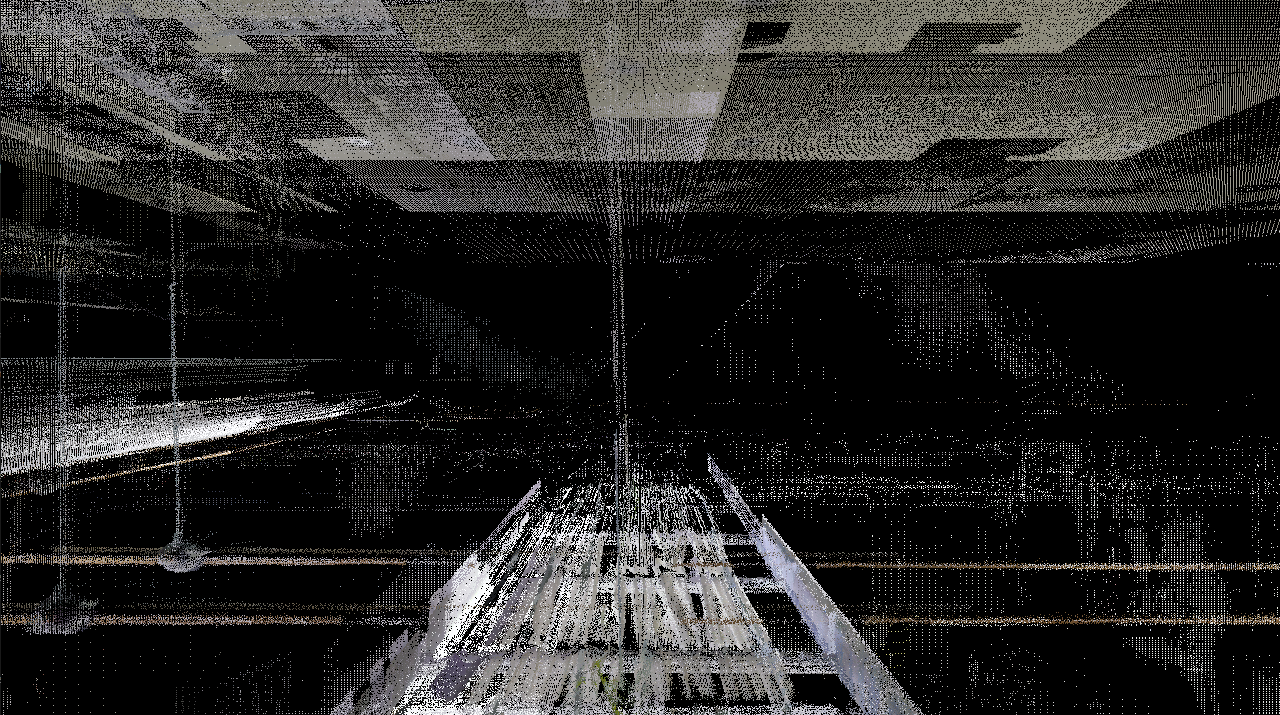
\includegraphics[width=0.75\textwidth]{tuloksia/ilmastointi_2M/ilmastointihuone_kaapelirata.png}
    \caption{Kahden miljoonan pisteen budjetin käyttäminen aiheuttaa ilmanvaihtohuone-pilvessä häiritseviä tarkkuustasojen välisiä eroja.}
    \label{lod_border}
\end{figure}

Laitossuunnitteluohjelmistossa pistepilven visualisointia voidaan kuitenkin jatkaa monen ruudun ajan, eikä pistebudjetin käyttäminen ole tarpeen. 3d-maisema pistepilvineen ja 2d-grafiikka, kuten kursori ja muut avustimet, voidaan piirtää näytönohjaimelle eri puskureihin. Näin on mahdollista piirtää uudestaan vain kursori, kun käyttäjä liikuttaa hiirtä, minkä jälkeen pistepilven visualisointia voidaan jatkaa siitä mihin viimeksi jäätiin. Oktettipuun solmujen järjestäminen tärkeyden mukaan on silti tarpeen. Kuten kuvasta \ref{img:worksite_vertailu} näkyy, järjestämisen ansiosta katselupistettä lähellä olevat mielenkiintoiset alueet tarkentuvat nopeammin.

%Mallinnustyössä pistepilvi täytyy usein piirtää useaan maisemaan samanaikaisesti. Käytännössä joudutaan harvoin tilanteeseen, jossa kamerat liikkuvat ja pistepilviä joudutaan päivittämään monessa maisemassa samaan aikaan. Kuitenkin olisi suotavaa, jos visualisoija piirtäisi ensin pistepilven yleiskuvan jokaiseen maisemaan, minkä jälkeen se kävisi maisemia läpi ja antaisi kullekin pienen aikasiivun pistepilven tarkentamiseen. Samoin usean pistepilven tapauksessa ei saisi käydä niin, että yksi pilvi piirretään täyteen tarkkuuteensa ennenkuin toista on edes aloitettu. 

\begin{figure}[t]
    \centering
    \subfloat[]{
        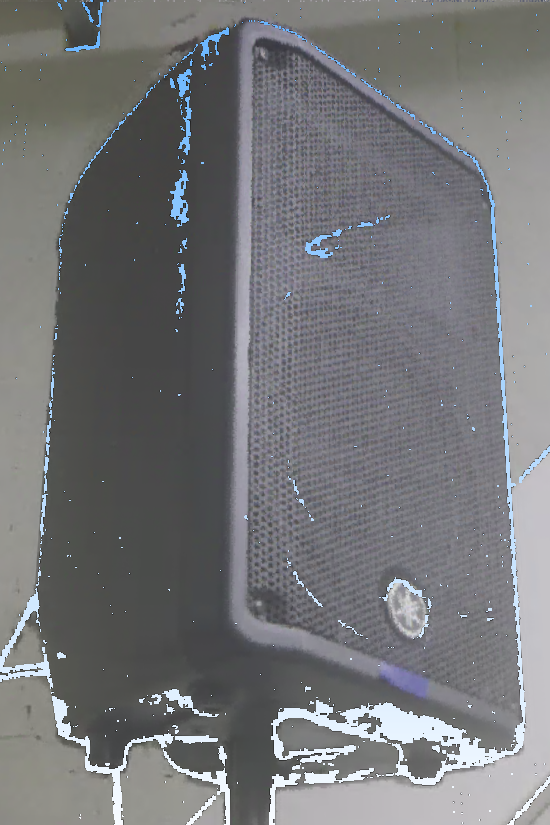
\includegraphics[width=.42\linewidth]{img/kaiutin2.png}
    }
    \subfloat[]{
        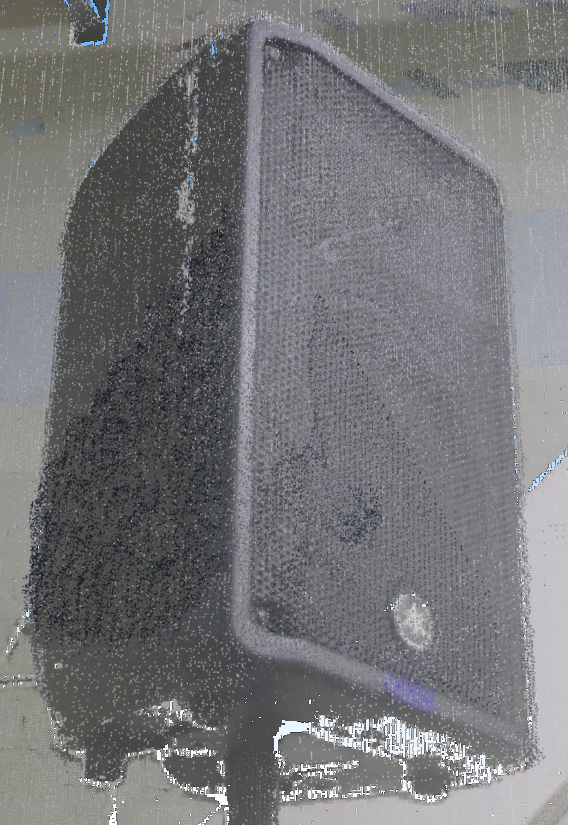
\includegraphics[width=.4338\linewidth]{img/kaiutin1.png}
    }
    \caption{Yksityiskohta panoraamakuvasta, joka on muodostettu (a) yhden laserkeilauksen sisältävästä ja (b) useita keilauksia sisältävästä pistepilvestä. Samojen pintojen mitatut värit vaihtelevat keilainten välillä. Pistepilvi on Elomatic Oy:n omaisuutta.}
    \label{img:kaiuttimet}
\end{figure}

Usealla laserkeilauksella mitattujen pisteiden yhdistäminen yhteen pistepilveen vaikuttaa negatiivisesti etenkin panoraamakuvien laatuun. Saman pinnan pisteet tallentuvat eri värisinä riippuen mistä kohtaa ne on mitattu. Tämä johtuu katselupisteiden välisistä eroista valaistuksessa, ja aiheuttaa kuvassa \ref{img:kaiuttimet} havainnollistettua ikävää häiriötä. Panoraamakuvaa piirtäessä olisikin hyödyllistä tietää, kuinka kaukaa kuvatasolle projisoitu piste on mitattu. Näin voitaisiin priorisoida pisteitä, jotka ovat lähellä keilaimen sijaintia.

Tutkielmassa esitelty oktettipuu ei suoraan sovellu putkien automaattiseen sovittamiseen pistepilveen luvussa \ref{laitossuunnittelu} esitellyillä tekniikoilla. Oktettipuu toki jakaa pistepilviä pienempiin osiin joita on helpompi käsitellä, mutta ongelmaksi muodostuu pisteiden jakautuminen puun jokaiselle tasolle. Jotta päästäisiin käsiksi tietyn alueen pisteisiin, täytyy käydä läpi kaikki solmut polulla juuresta alueen peittämiin lehtiin. Tehokkaampaa olisi, jos kaikki pisteet olisivat lehtisolmuissa, jolloin tarkasteltavissa solmuissa ei olisi halutun alueen ulkopuolisia pisteitä. Automaattista putkenreititystä varten olisikin ehkä kannattavaa järjestää pistepilvi johonkin toiseen tietorakenteeseen. 

Hierarkisen tietorakenteen rakentaminen vie aikaa eikä sen visualisointi ole yhtä nopeaa kuin pisteiden suoraviivainen piirtäminen. Laitossuunnitteluohjelmistossa käytettävien pistepilvien kokoluokka on harvoin teratavuja, joten muistien kasvaessa voisi olla kannattavaa hierarkisten tietorakenteiden kehittämisen sijaan keskittyä harventamaan pistepilveä niin, että se mahtuu näytönohjaimen muistiin ja käyttää jotakin ei-hierarkista tekniikkaa, joka käyttää näytönohjaimen rinnakkaislaskentatehoa mahdollisimman tehokkaasti.%, kuten luvussa \ref{ei-hier} esitellyt jatkuvat tarkkuustasot.

%Pisteiden hajauttaminen koko polulle juuresta lehtiin hidastaa myös pisteen valintaa pilvestä, mutta käytännössä valinta osoittautui riittävän nopeaksi.